\documentclass[a4paper,10pt]{scrartcl}
\usepackage[utf8]{inputenc}
\usepackage[T1]{fontenc}
\usepackage[naustrian]{babel}
\usepackage{lmodern}
\usepackage{graphicx}
\usepackage{hyperref}
%\usepackage{tabularx}
%\usepackage{amsmath}

%opening
\title{HCI Meilenstein 3}
\subtitle{Elektronisches Curriculum}
\author{Team 1 \\Pascal Attwenger, Philipp Hiermann, Sandra Markhart}

\begin{document}

\maketitle

\section{Usability Test Aufgaben}

\subsection{Aufgabe 1}

\subsubsection*{Ziel:}
 
Der User soll herausfinden welche Fächer er im 1. Semester absolvieren muss und kann.
 
\subsubsection*{Beschreibung:}

Du fängst nächstes Semester an Medieninformatik zu studieren. Für welche Fächer sollst du dich anmelden?
 
\subsection{Aufgabe 2}

\subsubsection*{Ziel:}

Der User soll seine Note abfragen.

\subsubsection*{Beschreibung:}

Du hast vor 2 Wochen die Vorlesungsprüfung zu VO Netzwerktechnologien abgelegt. Hast du bereits eine Note erhalten? Wenn ja welche?

\subsection{Aufgabe 3}

\subsubsection*{Ziel:}

Der User soll seinen Notendurchschnitt herausfinden.

\subsubsection*{Beschreibung:}

Du studierst an der Universität Wien und willst wissen ob du dich für ein Leistungsstipendium eignest. Das Stipendium verlangt einen Notendurchschnitt von
1,8. Kannst du ein Leistungsstipendium erhalten?


\section{Interviewleitfaden}

Usability Test Beispiel
•
Zielperson: Jugendliche
•
System: Webportal
•
Vorinterview
–
Erfahrungen mit ähnlichen Portalen
–
Erwartung vom Portal
•
Aufgaben mit jeweils Abschlussfragen
–
Zufriedenheit mit dem System
–
Verbesserungsvorschläge
•
Abschlussinterview
–
Allgemeine Eindrücke
–
Gut bzw. schlecht gefallen
–
Orientierung
–
Erwartungen erfüllt?

\subsection{Vorinterview}

\begin{itemize}
 \item Hast du schon Erfahrungen mit ähnlichen Systemen gesammelt?
 \item Welche Erwartungen hast du an das System?
\end{itemize}


\subsection{Fragen nach jeder Aufgabe}


\section{Abschlussinterview}




\section{Bericht}

\subsection{Aufgabe 1}

\subsection{Aufgabe 2}

\subsection{Aufgabe 3}

\subsection{Gesamteinschätzung}

\subsection{Verbesserungsvorschläge}

\section{Weiterentwickelter Prototyp}

\begin{description}
 \item[Url:] \url{http://wwwlab.cs.univie.ac.at/~a1151917/hci/}
 \item[Datei auf cewebs:]Meilenstein 3 - Team 1 - Webseite
\end{description}

Einerseits haben wir Verbesserungsvorschläge die bei der Präsentation des Meilensteins 2 aufgekommen sind, andererseits auch
die Verbesserungsvorschläge die wir aus den Interviews erhalten haben implementiert.

\subsection{Weiterentwicklung nach der Präsentation}

\subsubsection*{Statistik mit Anzahl der jeweiligen Noten}

Es gibt jetzt eine Statistik, in welcher zusätzlich die Anzahl der erbrachten Noten angezeigt wird.

\noindent\makebox[\textwidth]{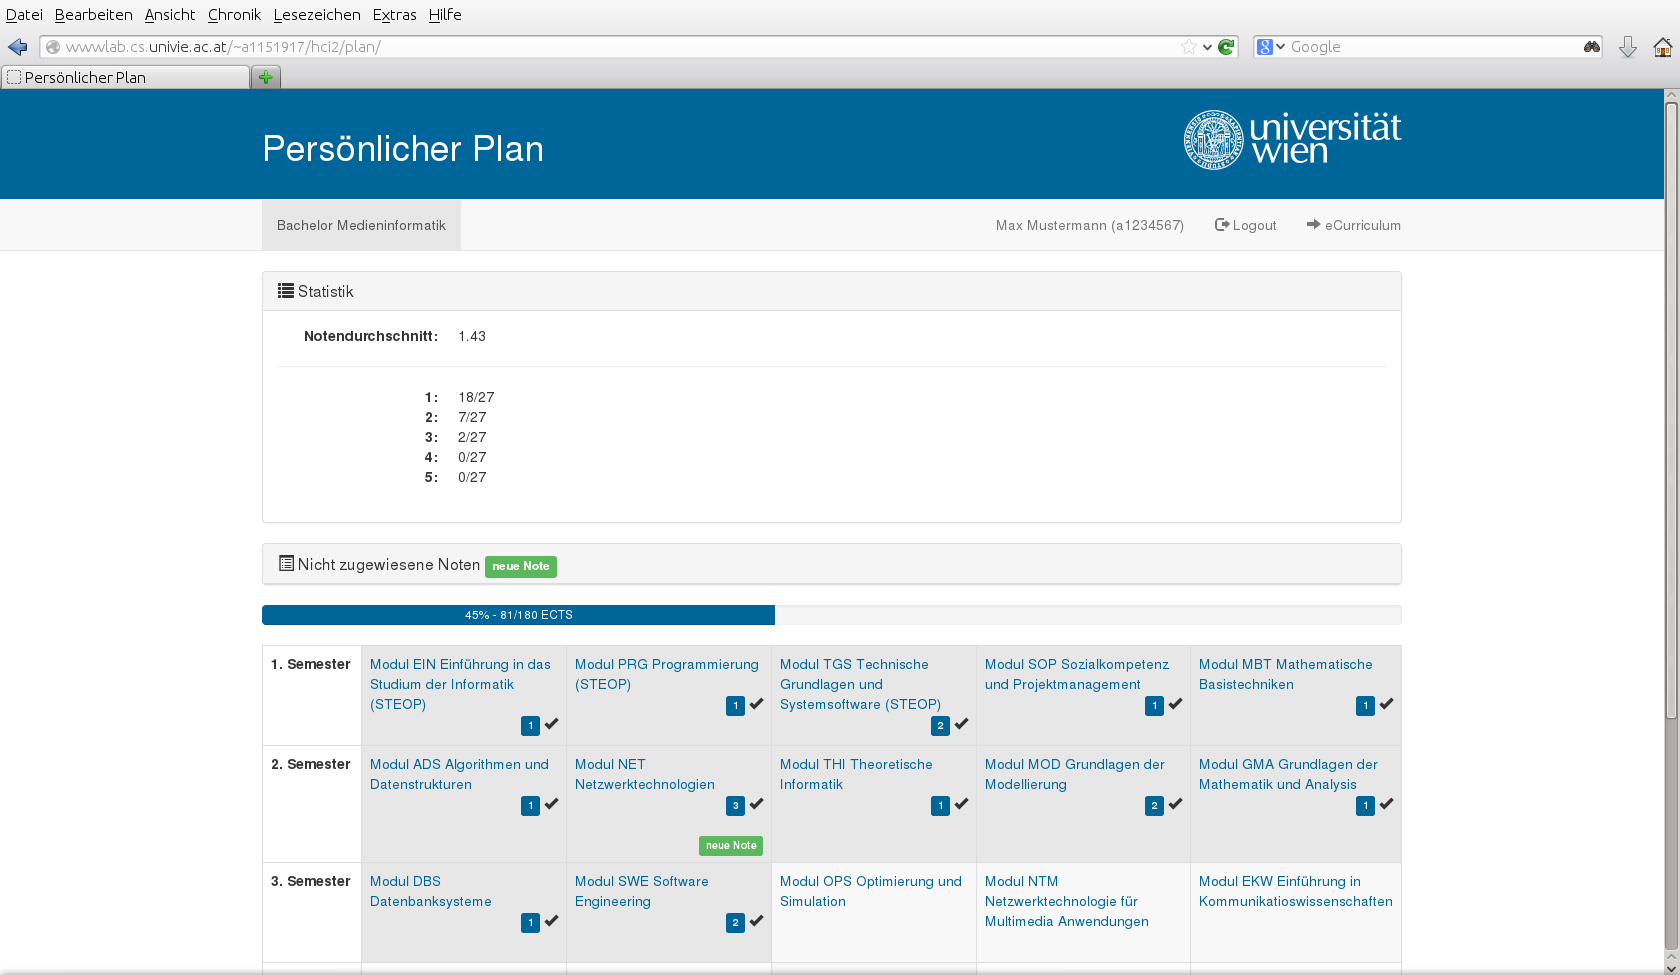
\includegraphics[width=\textwidth]{./verbesserung1.png}}
\medskip

\subsubsection*{Verlinkung zur Anmeldung zur Lehrveranstaltung}

Wenn eine Lehrveranstaltung noch nicht absolviert wurde, wird direkt ins Vorlesungsverzeichnis zum jeweiligen Modul verlinkt.

\noindent\makebox[\textwidth]{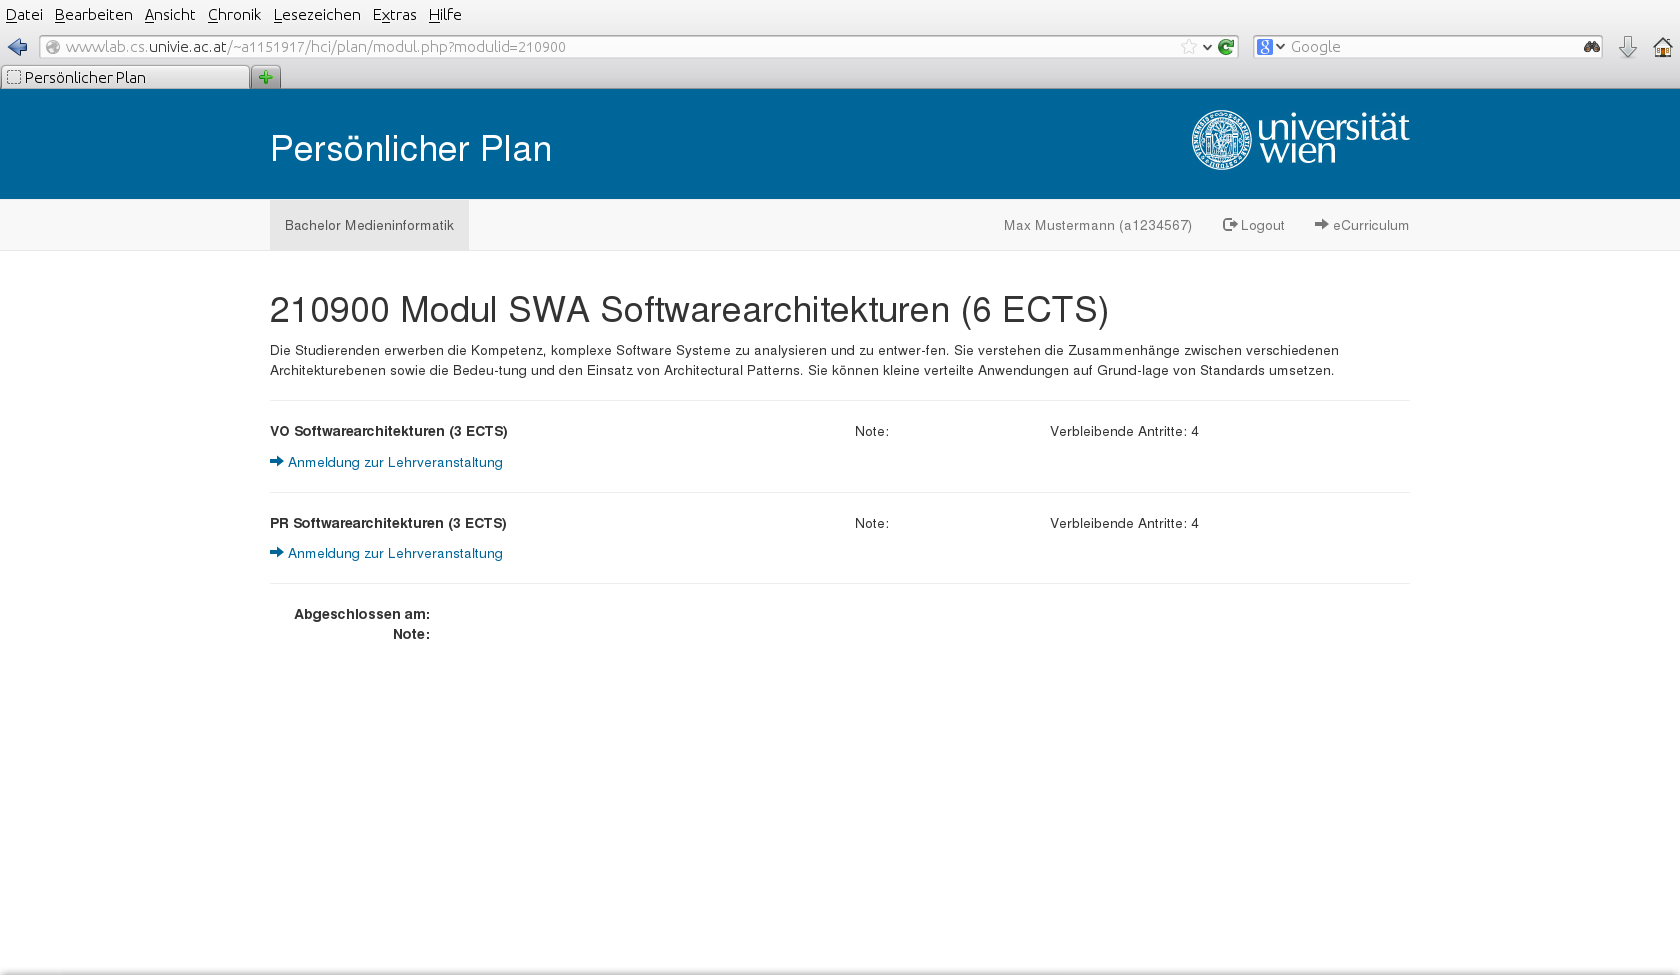
\includegraphics[width=\textwidth]{./verbesserung2.png}}
\medskip

\subsubsection*{Aufklappen aller Module im eCurriculum}




\subsection{Weiterentwicklung nach dem Interview}

\end{document}
